\makebox[\linewidth][c]{%
	\resizebox{1.3
	\textwidth}{!}{%
	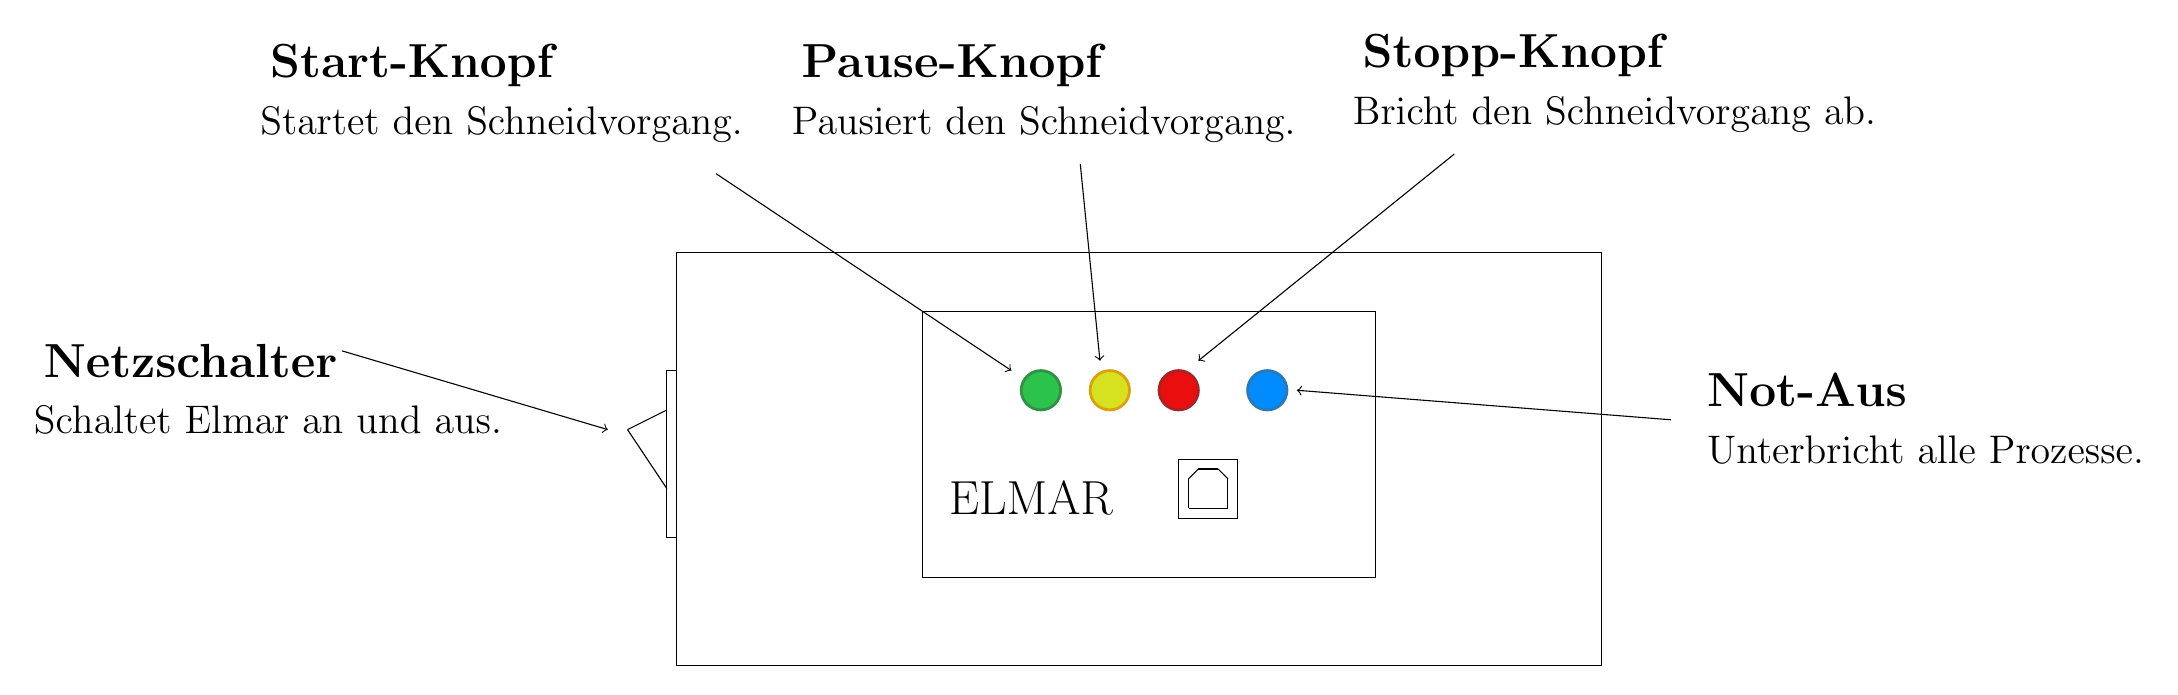
\begin{tikzpicture}
		\tikzstyle{every node}=[font=\fontsize{18.2pt}{23.7pt}\selectfont]
		
		\draw[fill={rgb,255:red,255; green,255; blue,255}, fill opacity=1] (3.25,14.375) rectangle (15,9.125);
		\draw[fill={rgb,255:red,255; green,255; blue,255}, fill opacity=1] (6.375,13.625) rectangle (12.125,10.25);
		\draw[fill={rgb,255:red,255; green,255; blue,255}, fill opacity=1] (3.25,12.875) rectangle (3.125,10.75);
		\draw (3.125,12.375) -- (2.625,12.125);
		\draw (2.625,12.125) -- (3.125,11.375);
		
		\draw[color={rgb,255:red,49; green,144; blue,70}, draw opacity=1, fill={rgb,255:red,44; green,195; blue,77}, fill opacity=1, line width=1pt] (7.875,12.625) circle (0.25cm);
		
		\draw[->] (3.75,15.375) -- (7.5,12.875);
		\draw[->] (15.875,12.25) -- (11.125,12.625);
		\draw[->] (8.375,15.5) -- (8.625,13);
		\draw[->] (-1,13.125) -- (2.375,12.125);
		\draw[->] (13.125,15.625) -- (9.875,13);
		
		\node[inner xsep=0.080cm, inner ysep=0.085cm, rounded corners=0.020cm, anchor=west] at (-2,16.75) {\textbf{Start-Knopf}};
		\node[inner xsep=0.080cm, inner ysep=0.085cm, rounded corners=0.020cm, anchor=west] at (4.75,16.75) {\textbf{Pause-Knopf}};
		\node[inner xsep=0.080cm, inner ysep=0.085cm, rounded corners=0.020cm, anchor=west] at (11.875,16.875) {\textbf{Stopp-Knopf}};
		\node[inner xsep=0.080cm, inner ysep=0.085cm, rounded corners=0.020cm, anchor=west] at (-4.875,13) {\textbf{Netzschalter}};
		
		\node[fill={rgb,255:red,255; green,255; blue,255}, fill opacity=1, text opacity=1, inner xsep=0.080cm, inner ysep=0.085cm, rounded corners=0.020cm, anchor=west] at (16.25,12.625) {\textbf{Not-Aus}};
		
		\node[font=\fontsize{14.2pt}{18.5pt}\selectfont, inner xsep=0.080cm, inner ysep=0.085cm, rounded corners=0.020cm, anchor=west] at (-5,12.25) {Schaltet Elmar an und aus.};
		\node[font=\fontsize{14.2pt}{18.5pt}\selectfont, inner xsep=0.080cm, inner ysep=0.085cm, rounded corners=0.020cm, anchor=west] at (-2.125,16) {Startet den Schneidvorgang.};
		\node[font=\fontsize{14.2pt}{18.5pt}\selectfont, inner xsep=0.080cm, inner ysep=0.085cm, rounded corners=0.020cm, anchor=west] at (11.75,16.125) {Bricht den Schneidvorgang ab.};
		\node[font=\fontsize{14.2pt}{18.5pt}\selectfont, inner xsep=0.080cm, inner ysep=0.085cm, rounded corners=0.020cm, anchor=west] at (4.625,16) {Pausiert den Schneidvorgang.};
		\node[font=\fontsize{14.2pt}{18.5pt}\selectfont, inner xsep=0.080cm, inner ysep=0.085cm, rounded corners=0.020cm, anchor=west] at (16.25,11.875) {Unterbricht alle Prozesse.};
		
		\draw[color={rgb,255:red,220; green,160; blue,13}, draw opacity=1, fill={rgb,255:red,214; green,226; blue,32}, fill opacity=1, line width=1pt] (8.75,12.625) circle (0.25cm);
		\draw[color={rgb,255:red,168; green,36; blue,36}, draw opacity=1, fill={rgb,255:red,235; green,14; blue,14}, fill opacity=1, line width=1pt] (9.625,12.625) circle (0.25cm);
		\draw[color={rgb,255:red,40; green,121; blue,188}, draw opacity=1, fill={rgb,255:red,0; green,140; blue,255}, fill opacity=1, line width=1pt] (10.75,12.625) circle (0.25cm);
		
		\draw (9.625,11.75) rectangle (10.375,11);
		\draw (9.875,11.625) -- (10.125,11.625);
		\draw (10.125,11.625) -- (10.25,11.5);
		\draw (9.875,11.625) -- (9.75,11.5);
		\draw (9.75,11.5) -- (9.75,11.125);
		\draw (10.25,11.5) -- (10.25,11.125);
		\draw (9.75,11.125) -- (10.25,11.125);
		
		\node at (7.75,11.25) {ELMAR};
		
	\end{tikzpicture}
}%
}